%\documentclass[aspectratio=43]{beamer}
\documentclass[t]{beamer}
\usetheme{ffmodern}  %% Themenwahl

\usepackage[ngerman]{babel} 
\usepackage[T1]{fontenc}    % richtige Silbentrennung
\usepackage[utf8]{inputenc} % Umlaute etc.!
\usepackage{eurosym}
\usepackage{tikz}
\usepackage{pgffor}

\usetikzlibrary{arrows,decorations.pathmorphing,backgrounds,fit,positioning,shapes.symbols,chains}

\title{Freifunk Hamburg}
\author{hamburg.freifunk.net}
\date{}
\license{CC-BY-3.0}

\begin{document}
\maketitle

\begin{frame}{Wat isn Freifunk\hl{?}}
    \begin{itemize}
        \item Kommunikationsinfrastruktur
        \item Community
        \item User
    \end{itemize}
\end{frame}

\begin{frame}{Dat is Freifunk\hl{!}}
    \begin{itemize}
        \item Frei
        \item Offen
        \item Neutral
        \item Dezentral
        \item Unabhängig
    \end{itemize}
\end{frame}

\begin{frame}{Wo denn\hl{?}}
    \begin{center}
        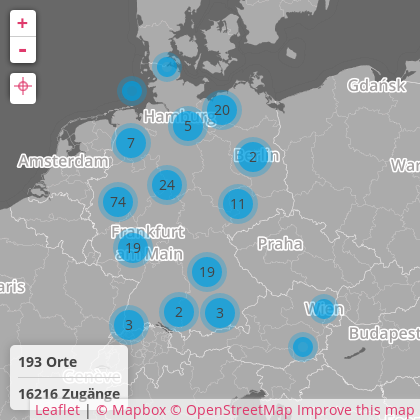
\includegraphics[width=.5\textwidth]{Bilder/community-map-2015-07-20}
    \end{center}
\end{frame}

\begin{frame}{Freifunk Hamburg\ANKER{}}
    \begin{itemize}
        \item Zweite Iteration
        \item Seit November 2012
        \item Loser Zusammenschluss
        \item Projekt im CCC Hamburg
        \item Etwa 860 Knoten
    \end{itemize}
\end{frame}

\foreach \index in {1, ..., 3} 
{
    \begin{frame}{Wie haut dat hin\hl{?}}
        \centering \includesvg[width=9cm]{netz-\index}
    \end{frame}
}

\begin{frame}{So is dat\hl{!}}
    \centering \includesvg[width=9cm]{netz-4-neu}
\end{frame}

\begin{frame}{Direkt von der Waterkant\hl{!}}
    \begin{itemize}
        \item map.hamburg.freifunk.net
    \end{itemize}
\end{frame}

\begin{frame}{Sicher dat\hl{?}}
    \begin{itemize}
        \item Keine Verschlüsselung über die Luft!
        \item Ungeschützter Datenverkehr ist gefährlich!
        \item Freifunk und Heimnetz sind getrennt
    \end{itemize}
\end{frame}

\begin{frame}{Geiht dat klar\hl{?}}
    \begin{itemize}
        \item Störerhaftung
        \item Verschlüsselte Verbindung zu den Gateways
        \item Privatanschlüsse nicht zurückverfolgbar
    \end{itemize}
\end{frame}

\begin{frame}{Dat funkt so\hl{!}}
    \begin{itemize}
        \item Chat
        \item Blogs
        \item News
        \item Verbindung zu anderen Städten
        \item Dein Dienst hier!
    \end{itemize}
\end{frame}

\begin{frame}{Wat geiht\hl{?}}
    \includegraphics[width=\textwidth]{Bilder/esmarch95}
    
    \begin{itemize}
        \item Richtfunk-Backbone im Aufbau
        \item Sechs Standorte stehen
        \item Weitere in Planung
    \end{itemize}
\end{frame}

\begin{frame}{Mook wat\hl{!}}
    \begin{itemize}
        \item Rede über Freifunk
        \item Stelle Router auf
        \item Betreibe eigene Dienste
        \item Bring Dich ein
        \item Komm zum Treffen
        \begin{itemize}
            \item Montag 19:00 beim CCCHH
            \item Freitag 19:30 beim Attraktor e. V.
        \end{itemize}
    \end{itemize}
\end{frame}

\begin{frame}{Klönen\hl{?}}
    \begin{itemize}
        \item hamburg.freifunk.net
        \item @FreifunkHH
        \item irc://irc.hackint.net/ffhh
    \end{itemize}
    %\includegraphics[width=0.5\textwidth]{Bilder/cc-by}
\end{frame}

\begin{frame}{}
    \vspace{1.6cm}
    \centering \includesvg[width=4cm]{in-hamburg-funkt-man-frei}
    \vspace{0.8cm}

    {\Huge\bf Dann man tau\hl{!}}
\end{frame}

\end{document}
